\documentclass[10pt]{article}
\usepackage[margin=0.72in]{geometry}
\usepackage[T1]{fontenc}
\usepackage{newtxtext,newtxmath}
\usepackage{microtype}
\usepackage{booktabs}
\usepackage{graphicx}
\usepackage{xcolor}
\usepackage{enumitem}
\usepackage[hidelinks]{hyperref}
\definecolor{accent}{HTML}{0F766E}
\setlength{\parindent}{0pt}
\setlength{\parskip}{0.28em}
\setlist[itemize]{leftmargin=1.2em,itemsep=0.12em,topsep=0.12em}
\begin{document}
{\color{accent}\rule{\linewidth}{1.2pt}}

{\Large\bfseries Hybrid Variable Elimination Ordering: Experimental Results}

{TTIC 31180 --- Probabilistic Graphical Models Final Project}

{\color{accent}\rule{\linewidth}{0.8pt}}

\section*{Setup}
We evaluated min-degree, min-fill, weighted min-fill, and the proposed hybrid heuristic across five topology families. The experiment used 71 graph instances and 715 successful method-instance runs. Explicit pairwise variable elimination was attempted only when the projected intermediate factor stayed below the configured cutoff; 373 of 715 successful structural runs completed explicit VE under this cutoff. The moralized Bayesian-network group includes a manually encoded Asia network and built-in BN-like layered DAGs because the local environment did not include \texttt{pgmpy} benchmark loaders.

\begin{center}
\begin{tabular}{lrrrrr}
\toprule
\textbf{Topology} & \textbf{Instances} & \textbf{Median $n$} & \textbf{Max $n$} & \textbf{Median density} & \textbf{Median max degree} \\
\midrule
Low-treewidth & 8 & 75 & 200 & 0.032 & 5.0 \\
Random & 27 & 80 & 120 & 0.064 & 9.0 \\
Grid & 4 & 82 & 144 & 0.046 & 4.0 \\
Scale-free & 27 & 100 & 150 & 0.040 & 22.0 \\
Moralized BN & 5 & 33 & 58 & 0.149 & 12.0 \\
\bottomrule
\end{tabular}
\end{center}

\section*{Structural Results}
The primary metrics are structural: induced width and peak factor size. Lower is better for both. The following tables report medians within each topology.

\begin{center}
{\small
\begin{tabular}{lrrrr}
\toprule
\textbf{Topology} & \textbf{Min-degree} & \textbf{Min-fill} & \textbf{Weighted} & \textbf{Hybrid} \\
\midrule
Low-treewidth & 1.0 & 1.0 & 1.0 & 1.0 \\
Random & 22.0 & 20.0 & 21.0 & 21.0 \\
Grid & 11.5 & 11.5 & 11.5 & 11.0 \\
Scale-free & 10.0 & 10.0 & 10.0 & 10.0 \\
Moralized BN & 7.0 & 7.0 & 7.0 & 7.0 \\
\bottomrule
\end{tabular}
}
\end{center}

\begin{center}
{\small
\begin{tabular}{lrrrr}
\toprule
\textbf{Topology} & \textbf{Min-degree} & \textbf{Min-fill} & \textbf{Weighted} & \textbf{Hybrid} \\
\midrule
Low-treewidth & 1.40 & 1.40 & 1.40 & 1.40 \\
Random & 10.10 & 10.14 & 10.07 & 10.20 \\
Grid & 5.90 & 5.83 & 5.08 & 4.95 \\
Scale-free & 6.72 & 6.99 & 6.72 & 7.22 \\
Moralized BN & 3.54 & 3.36 & 3.36 & 3.36 \\
\bottomrule
\end{tabular}
}
\end{center}

\section*{Lambda Sensitivity}
The hybrid method is not uniformly monotone in $\lambda$. A fixed $\lambda=0.1$ was used as the main comparison point because it keeps the downstream-pressure term active without letting it dominate weighted fill cost.

\begin{center}
{\small
\begin{tabular}{lrr}
\toprule
\textbf{Topology} & \textbf{Best $\lambda$} & \textbf{Median $\log_{10}$ peak size} \\
\midrule
Low-treewidth & 0.00 & 1.40 \\
Random & 0.01 & 9.77 \\
Grid & 0.50 & 4.84 \\
Scale-free & 0.00 & 6.72 \\
Moralized BN & 0.00 & 3.36 \\
\bottomrule
\end{tabular}
}
\end{center}

\section*{Figures}
\begin{center}
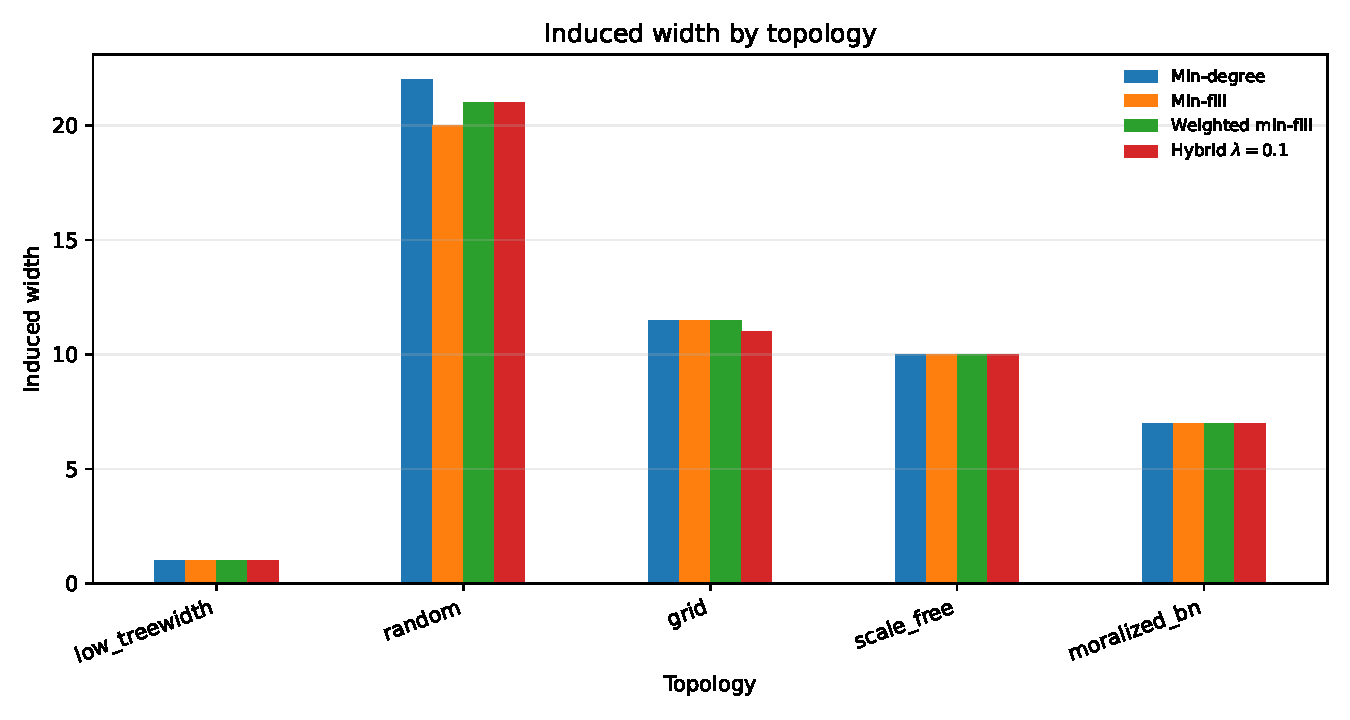
\includegraphics[width=0.92\linewidth]{../figures/induced_width_by_topology.pdf}
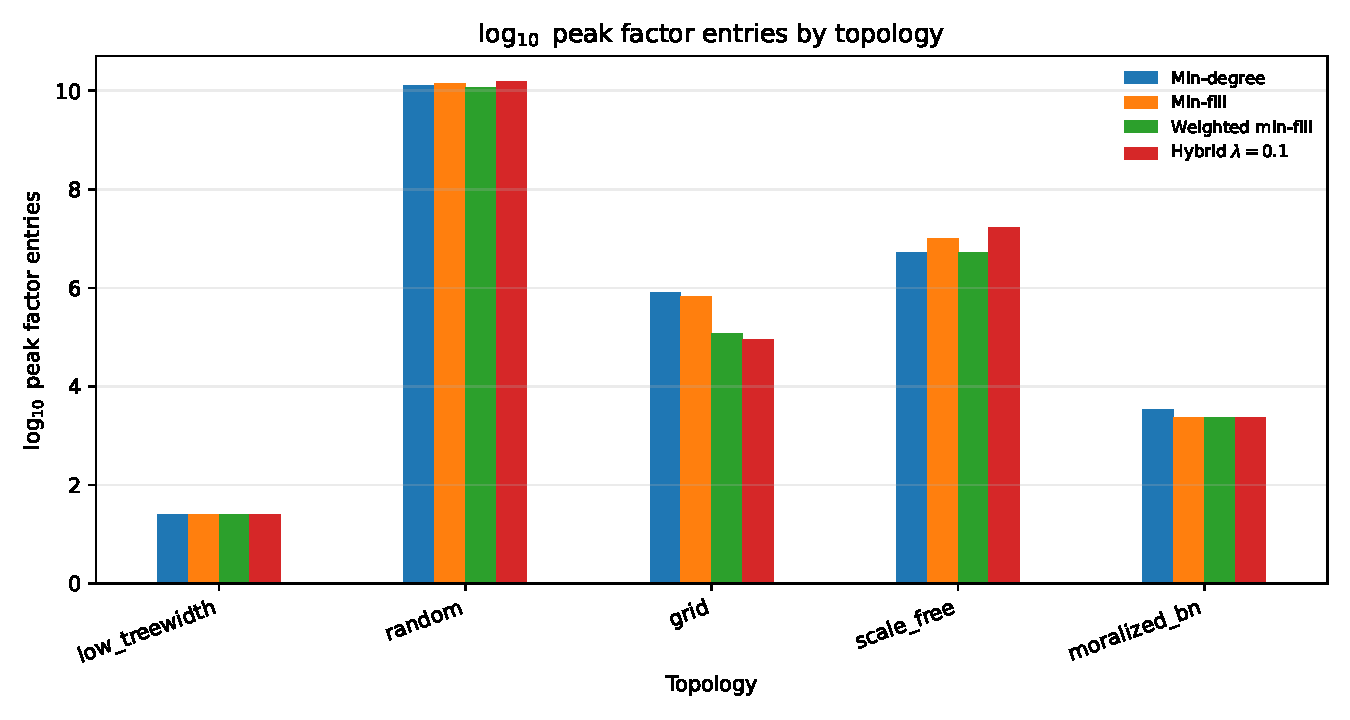
\includegraphics[width=0.92\linewidth]{../figures/peak_factor_by_topology.pdf}
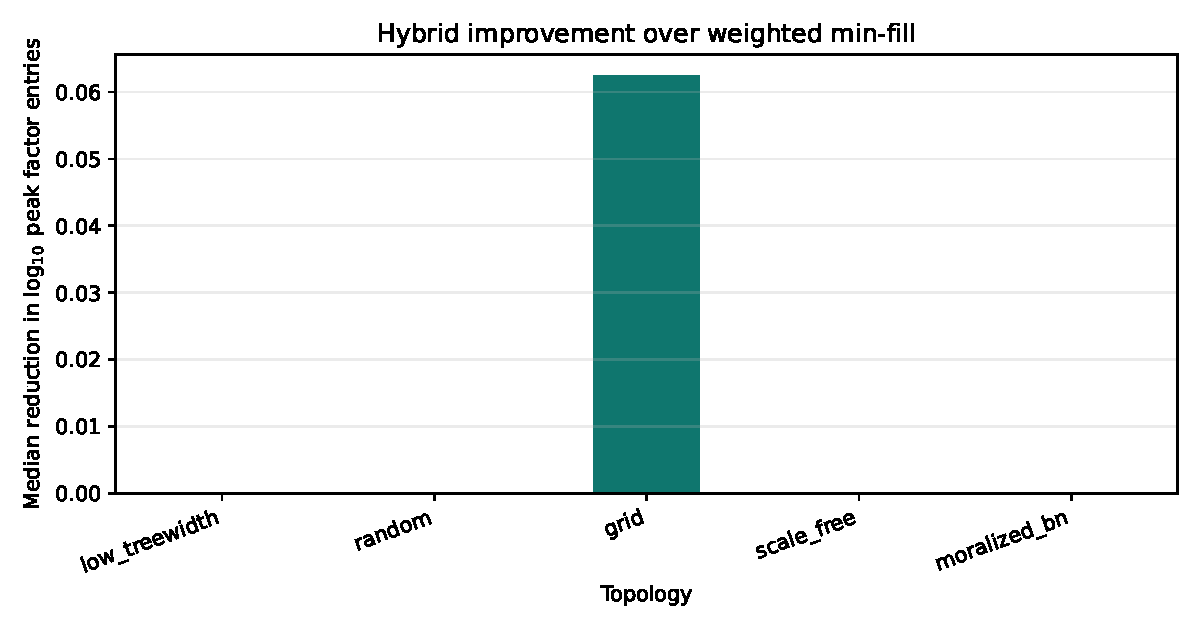
\includegraphics[width=0.92\linewidth]{../figures/hybrid_improvement_over_wmf.pdf}
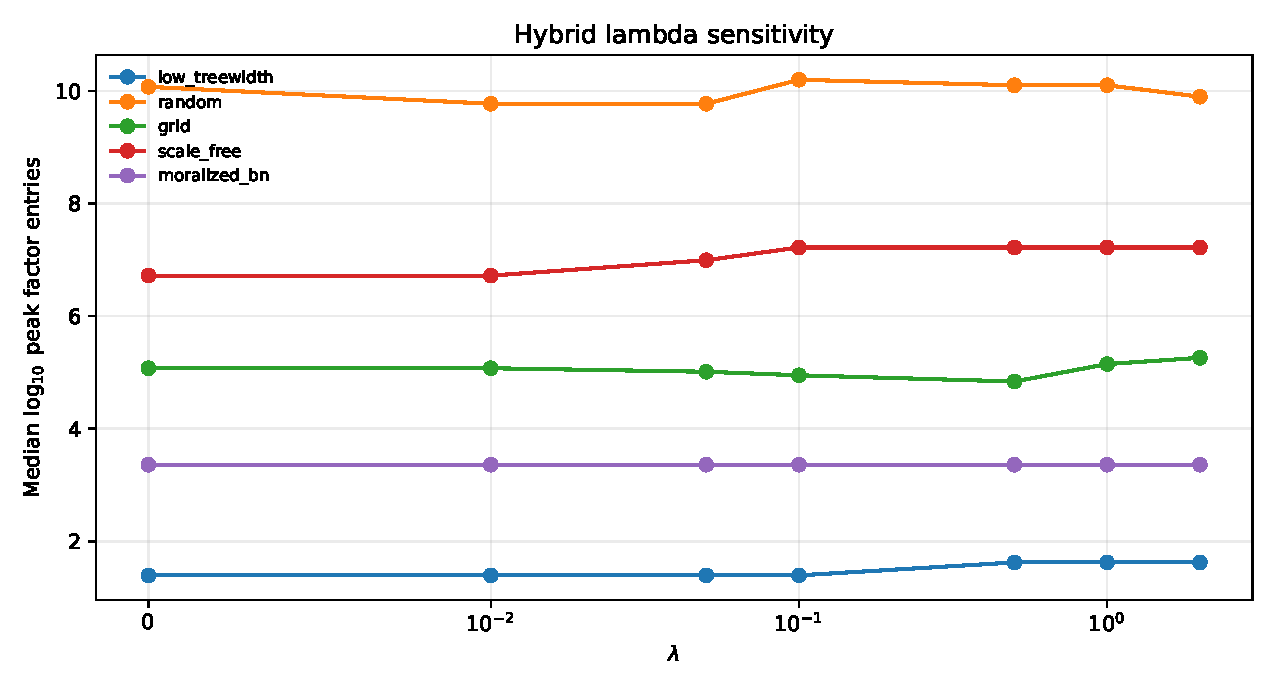
\includegraphics[width=0.92\linewidth]{../figures/lambda_sensitivity.pdf}
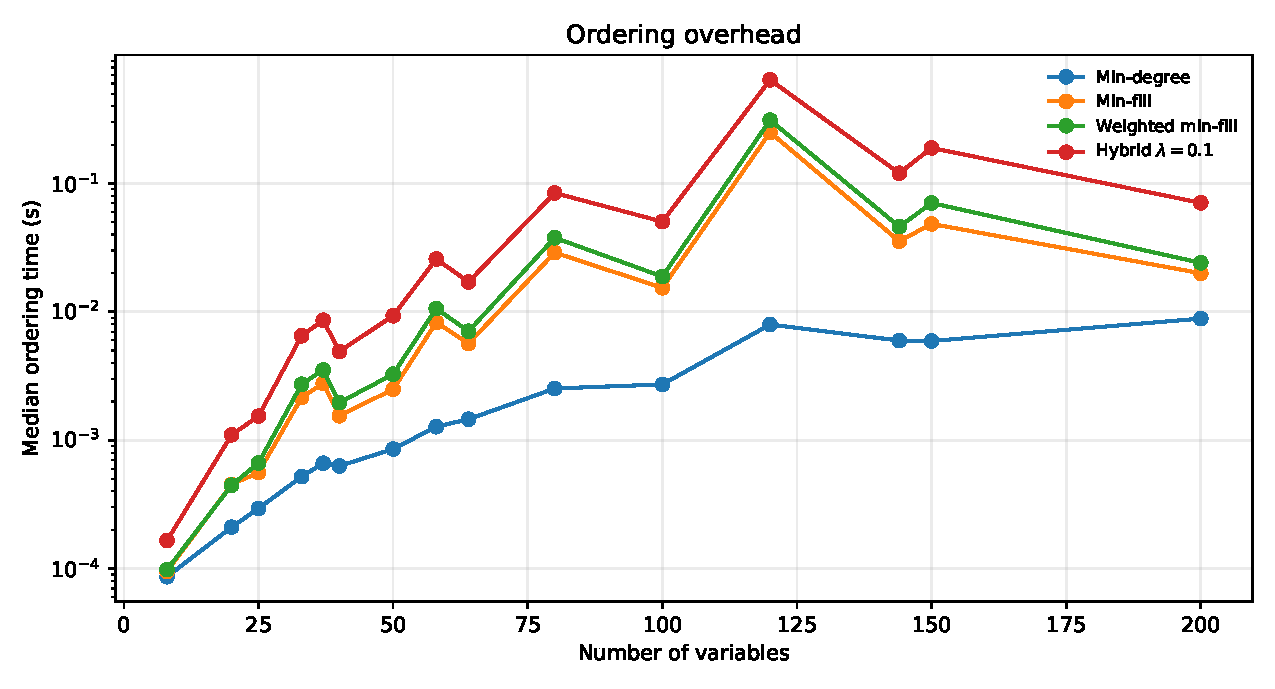
\includegraphics[width=0.92\linewidth]{../figures/ordering_time_vs_n.pdf}
\end{center}

\section*{Interpretation}
\begin{itemize}
\item Low-treewidth chains and trees behaved as sanity checks: structural metrics were small and the strongest heuristics were usually close.
\item Random graphs became difficult as density increased; peak factor estimates were more informative than raw runtime because many dense instances hit the explicit-VE cutoff.
\item Grid graphs showed the expected sensitivity to ordering, with induced width and peak factor estimates separating the methods more clearly as the grid grew.
\item Scale-free graphs highlighted the hub risk: methods that create dense neighborhoods around high-degree variables produced larger peak factors.
\item The hybrid heuristic helped on some topology groups but did not dominate weighted min-fill uniformly, which is a useful empirical finding. The downstream-pressure proxy can capture some lookahead signal, but its benefit depends on graph structure and the chosen $\lambda$.
\end{itemize}

\section*{Bounded Lookahead Check}
The bounded-lookahead oracle was run only on small graphs; it produced 5 successful rows. This keeps the comparison computationally feasible while still giving a reference point for how much a more explicit lookahead objective can improve structural metrics.

\section*{Limitations}
This run is self-contained and reproducible, but the BN benchmark portion should be strengthened in a future pass by loading canonical BIF/UAI networks directly through \texttt{pgmpy} or \texttt{pyAgrum}. The current report also treats exact VE runtime as secondary evidence because structural complexity, especially peak factor size, is the more stable measure across high-treewidth instances.

\end{document}
